\documentclass[12pt,letterpaper]{article}


\newcommand{\studentname}{Ben Bassett}

\title{\textsc{Lab 12: Birefringent Tape}}
\newcommand{\shorttitle}{Birefringent Tape}

\newcommand{\course}{PHY310}
\newcommand{\labdate}{11-26-2024}

%------------------------------------------------------------------------------------------------------------

\usepackage[letterpaper,left=1in,right=1in,bottom=1in,top=1in]{geometry}
\usepackage{fancyhdr}
\usepackage{subfigure}
\usepackage{graphicx}
\usepackage{amsmath}
\DeclareMathOperator{\sinc}{sinc}
\usepackage{cleveref}
\usepackage{booktabs}
\usepackage[british]{babel}
\usepackage[square,comma,numbers,sort&compress]{natbib}
\usepackage{csvsimple}
\usepackage{graphicx}
\usepackage{pgfplotstable}
\usepackage{textcomp,gensymb}
\usepackage{array}
\usepackage{tabu}
\usepackage{multirow}
\usepackage{url}
\usepackage{lipsum}
\usepackage{dsfont}
\usepackage{fontspec}
\pgfplotsset{compat=1.9}% supress warning
\begin{document}

%------------------------------------------------------------------------------------------------------------

\setlength{\parindent}{1em}
\setlength{\parskip}{0.5em}
\author{\course~Lab Journal \\ \\ \studentname} % \,\& \labpartner}
\date{\labdate}

% \setmainfont{Wingdings-Regular.ttf}


\renewcommand\abstractname{Summary}

\pagestyle{fancy}
\fancyhead{}
\fancyhead[l]{\course:~\shorttitle}
\fancyhead[r]{\studentname}
\fancyfoot{}
\fancyfoot[C]{\thepage}
\renewcommand{\headrulewidth}{0pt}
\renewcommand{\footrulewidth}{0pt}

\renewcommand\bibname{References}

%------------------------------------------------------------------------------------------------------------

\renewcommand\abstractname{Abstract}
\maketitle

% COMMENT IN IF ASKED TO SUBMIT REPORT WITH ABSTRACT
\begin{abstract}

In this lab we used the attributes of birefringence to measure the $\Delta n$ value of a piece of polypropylene packing tape by rotating it between two polarizers (either perpendicular or parallel) and measuring the intensity of a laser beam passed through the setup at various rotations. We computed the phase change across the rotation, and from that could compute the value of the birefringence.

\end{abstract}

\section{Experimental Apparatus}

Materials given were 650 nm red laser diode, two polarizers, a light sensor with various apertures, and a rotation sensor connected to an aperture covered with packing tape. Our setup is illustrated in Figure \ref{fig:setup}.

\begin{figure}[ht]
    \centering
    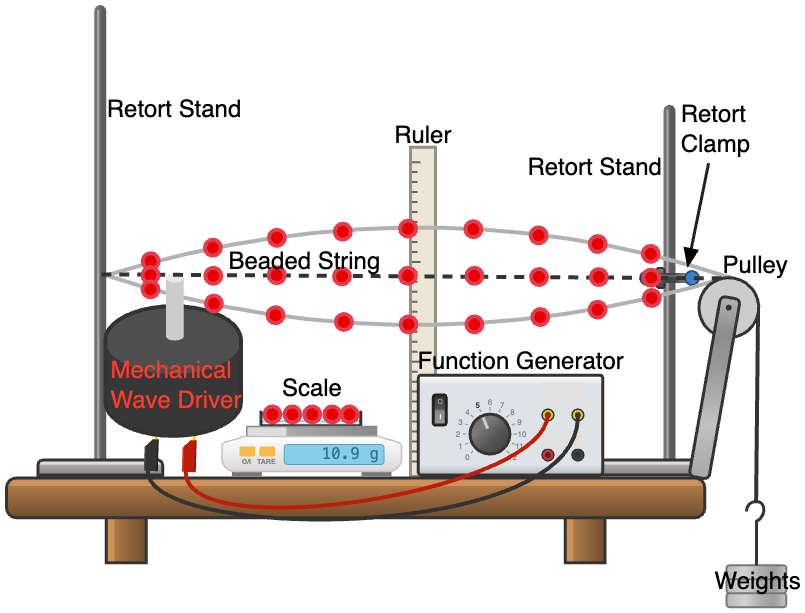
\includegraphics[width=3.7in]{images/setup.png}
    \caption{The final optics track setup}
    \label{fig:setup}
\end{figure}

% \pagebreak
\section{Procedure}

We ran the experiment twice—once when the two polarizers were perpendicular to each other so that almost no light was let through, and once when they were parallel so as much light as possible was let through. We calibrated these without the tape in the system, and by observing the luminance on the light sensors as we rotated the polarizers. The aperture was set to 10\%.

Once each run had been calibrated, we inserted the tape and zeroed the rotation sensor. Then we recorded data at 20 samples per second for 60 seconds, all while slowly rotating the tape by hand. Logger Pro recorded the luminance and rotation values throughout, and we saved it as a csv for later processing.

\section{Results}

We took the RMS of our data and used the midpoint to find the max and min of the data. Because some of the data was very noisy from performing the experiment in a bright room with a large aperture, I took the 95th and 5th percentile of the data to avoid some weird extra spikes. See the dotted lines in Figures 2-4

\begin{equation}
    \cos\phi=\frac{\text{min}(I_A)-\text{max}(I_B)}{\text{min}(I_A)+\text{max}(I_B)}
\end{equation}

\begin{figure}[ht]
    \centering
    \includegraphics[width=4in]{images/parallel10.png}
    \caption{Parallel polarizers with the 10\% aperture}
    \label{fig:||10}
\end{figure}

\begin{figure}[ht]
    \centering
    \includegraphics[width=4in]{images/perpindicular10.png}
    \caption{Perpendicular polarizers with the 10\% aperture}
    \label{fig:||10}
\end{figure}

\begin{figure}[ht]
    \centering
    \includegraphics[width=4in]{images/parallelplastic.png}
    \caption{Parallel polarizers with the thin plastic aperture}
    \label{fig:||10}
\end{figure}

The second data in Figure 4 was taken with the aperture set to thin plastic, so it was harder to ambient light to make much of a difference, creating the noisy data in Figure 2. However, as we neglected to run the perpendicular setup with the plastic aperture, we won't use it. 

We plug in the max and min from Figures 2 and 3 into Equation 1:

\begin{equation*}
    \phi = \cos^{-1}\left(\frac{73393.50 - 7947.35}{73393.50 + 7947.35}\right)
\end{equation*}

Computing this, we find that $\phi = \mathbf{36.43 \pm 0.00} \textbf{ degrees}$. This tells us the difference in path for the light introduced by the tape. This phase difference is given by

\begin{equation}
    \phi=2\pi\frac{\Delta nd}{\lambda}
\end{equation}

Since we know our one layer of tape was 1.6 mil thin (0.00004064 meters), we can compute $\Delta n$, which from the values given above we found to be $\mathbf{1.618\times10^{-3}}$, a unitless value

\section{Conclusions}

Figure 5 is a chart of results from \textit{Quantitative measurement of birefringence in transparent films across the visible spectrum}
by Aaron D. Slepkov, which makes our $\Delta n = \mathbf{1.618\times10^{-3}}$ value seem quite realistic! Birefringence works!

\begin{figure}[ht]
    \centering
    \includegraphics[width=4in]{images/values.jpg}
    \caption{Professionally measured birefringence values}
    \label{fig:real}
\end{figure}

% \bibliographystyle{unsrtnat}
% \bibliography{references}

\end{document}
